\documentclass[9pt,twocolumn]{article}
\usepackage[margin=0.68in,columnsep=0.22in]{geometry}
\usepackage{graphicx}
\usepackage{microtype}
\usepackage[hidelinks]{hyperref}
\setlength{\parindent}{1em}
\setlength{\parskip}{0pt}
\title{\vspace{-1.8em}SeraEdit: Reliable Language-Guided MusicXML Editing through Structured Score Patches\vspace{-0.7em}}
\author{Anonymous submission}
\date{}

\begin{document}
\maketitle
\vspace{-1.4em}
\begin{abstract}
Natural-language score editing is attractive for notation workflows, but asking a language model to rewrite an entire MusicXML document can damage unrelated notes, voices, and notation relations. We present SeraEdit, a language-guided editing layer built around a canonical score document and a versioned, source-bound ScorePatch. Each patch declares target and protected scopes, stable event identifiers, preconditions, and typed operations. A transactional pipeline validates schema, structure, measure duration, notation relations, protected content, and MusicXML round trips before committing, with bounded repair and explicit refusal on failure. We define a 120-task benchmark protocol spanning pitch, rhythm, harmony, voice, notation, structure, compound, and conflicting edits, and compare full-score rewrite, patch-only, and the complete pipeline using deterministic task and preservation metrics. \textbf{[RESULT TO BE INSERTED FROM FORMAL LIVE EXPERIMENT.]}
\end{abstract}

\section{Introduction}
MusicXML is an open interchange format for digital sheet music~\cite{good2021musicxml}, but valid XML alone does not guarantee that a local edit preserved unrelated musical material. Language models can process text-compatible symbolic representations~\cite{yuan2024chatmusician}; evaluations nevertheless report weaknesses in multi-step musical reasoning~\cite{zhou2024reason}. SeraEdit treats model output as a proposed transaction rather than a replacement score.

Our contributions are limited to (1) a versioned structured ScorePatch bound to a source fingerprint; (2) a validation, protected-scope, repair/reject, and transactional application pipeline; and (3) a paired benchmark protocol comparing full rewrite, patch only, and the complete pipeline.

\section{Related Work}
MusicXML supplies the exchange representation, while music21 demonstrates programmatic symbolic-score analysis~\cite{cuthbert2010music21}. ChatMusician studies symbolic understanding and generation, not preservation-guaranteed local MusicXML editing. \emph{Not that Groove} directly studies zero-shot instruction-driven MIDI drum editing with programmatic tests~\cite{zhang2025groove}; SeraEdit focuses on staff notation, MusicXML round trips, protected scopes, and rollback. CodeEditorBench motivates evaluating editing separately from generation~\cite{guo2024codeeditorbench}.

\section{Method}
MusicXML is imported into one authoritative ScoreDocument. Stable event IDs, exact rational/tick positions, and SHA-256 fingerprints bind import, patch, preview, result, playback, and export. ScoreScope selects measures, parts, staffs, voices, event IDs, time ranges, and exclusions. A separate protected scope defines content that must not change.

A ScorePatch contains its version, source score and fingerprint, instruction, target/protected scopes, preconditions, expected effects, provenance, and typed operations. Application performs fingerprint, schema, selector, structural, duration, notation-relation, protected-scope, and MusicXML round-trip checks on a clone before commit. Deterministic repair precedes at most two model repair attempts; every attempt and added cost is retained. Unsupported or still-invalid edits are rejected with the original score intact.

\begin{figure}[t]
  \centering
  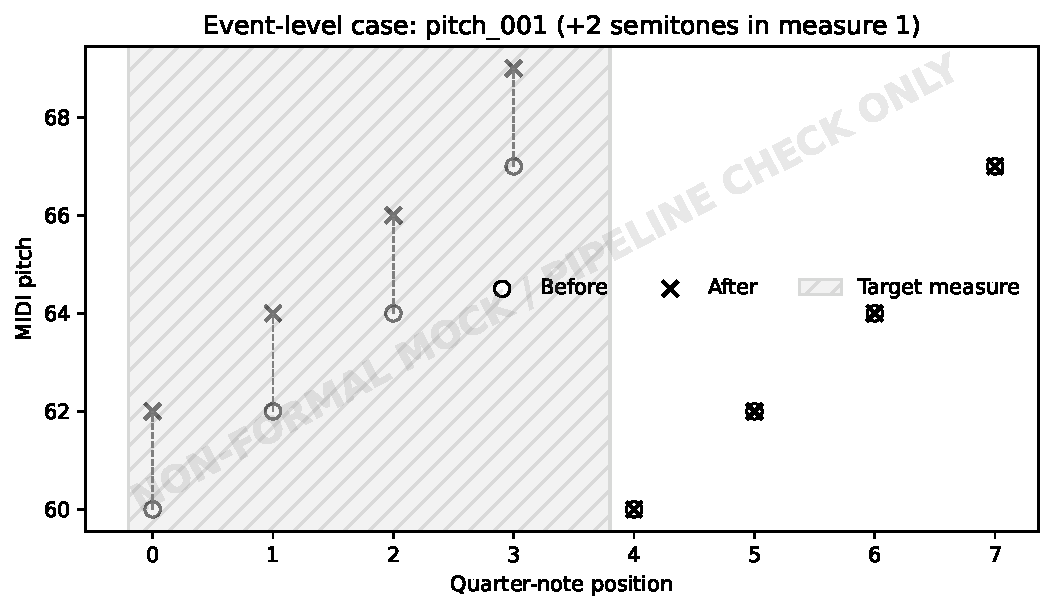
\includegraphics[width=\columnwidth]{../figures/score_edit_case_pitch_001.pdf}
  \caption{Deterministic benchmark case: target-measure events move by two semitones while protected events remain unchanged. This event plot is not an engraving-quality score rendering.}
  \label{fig:case}
\end{figure}

\section{Evaluation Protocol}
The Core protocol contains 120 tasks over 20 short synthetic or license-safe scores, spanning ten categories. Each task has target and protected scopes, deterministic constraints, and either a gold patch or explicit refusal target. Automatic validation passes all generated tasks; all remain marked \texttt{pending\_human\_review}.

Conditions are (A) complete MusicXML rewrite; (B) ScorePatch generation with schema parse and basic apply only; and (C) Sera Full. Metrics cover XML validity, patch parsing, task/constraint success, preservation, minimality, refusal, repair, latency, tokens, and cost. Paired analysis uses bootstrap confidence intervals, exact McNemar tests~\cite{mcnemar1947}, Wilcoxon signed-rank tests~\cite{wilcoxon1945}, effect sizes, and Holm correction~\cite{holm1979}.

\section{Results and Analysis}
\textbf{[RESULT TO BE INSERTED FROM FORMAL LIVE EXPERIMENT.]}

The current 360-run deterministic mock check verifies execution, cache/resume, evidence retention, metric recomputation, statistics, and paper-asset generation. It is not model-performance evidence and its scores are intentionally excluded here.

\section{Limitations and Conclusion}
The benchmark uses short symbolic excerpts and does not measure engraving or composition quality. Human review and cross-application MusicXML testing remain necessary. Provider versions may drift, and bounded repair may reject feasible edits. SeraEdit is an intelligent editing and collaboration layer over professional notation environments, not a replacement for MuseScore, Sibelius, or musical judgment.

\begin{thebibliography}{9}
\bibitem{good2021musicxml} M. Good, ed., ``MusicXML 4.0,'' W3C Music Notation Community Group Final Report, 2021.
\bibitem{cuthbert2010music21} M. S. Cuthbert and C. Ariza, ``music21: A toolkit for computer-aided musicology and symbolic music data,'' in \emph{ISMIR}, 2010, pp. 637--642.
\bibitem{yuan2024chatmusician} R. Yuan et al., ``ChatMusician: Understanding and generating music intrinsically with LLM,'' \emph{Findings of ACL}, 2024.
\bibitem{zhou2024reason} Z. Zhou et al., ``Can LLMs `reason' in music?'' in \emph{ISMIR}, 2024.
\bibitem{zhang2025groove} L. Zhang, ``Not that Groove: Zero-shot symbolic music editing,'' arXiv:2505.08203, preprint, 2025.
\bibitem{guo2024codeeditorbench} J. Guo et al., ``CodeEditorBench: Evaluating code editing capability of large language models,'' arXiv:2404.03543, 2024.
\bibitem{mcnemar1947} Q. McNemar, ``Note on the sampling error of the difference between correlated proportions or percentages,'' \emph{Psychometrika}, vol. 12, pp. 153--157, 1947.
\bibitem{wilcoxon1945} F. Wilcoxon, ``Individual comparisons by ranking methods,'' \emph{Biometrics Bulletin}, vol. 1, pp. 80--83, 1945.
\bibitem{holm1979} S. Holm, ``A simple sequentially rejective multiple test procedure,'' \emph{Scandinavian Journal of Statistics}, vol. 6, pp. 65--70, 1979.
\end{thebibliography}
\end{document}
